% Template for ApJ-type papers

\documentclass[12pt,preprint]{emulateapj}

\usepackage{rotating}
\usepackage{amssymb,amsmath}
\usepackage{graphicx}%[subfloat]
\usepackage{natbib}
\usepackage{subfig}
\usepackage{multirow}
\citestyle{aa}
\bibliographystyle{apj_w_etal}

\newcommand{\vect}[1]{\mathbf{#1}}
\newcommand{\xad}{\vect{x}}

\newcommand{\vdag}{(v)^\dagger}
\newcommand{\myemail}{jaguirre@nrao.edu}
\newcommand{\lsim}{{_{<}\atop^{\sim}}}
\newcommand{\gsim}{{_{>}\atop^{\sim}}}
\newcommand{\etal}{{et al.\/}}
\newcommand{\ie}{{\em ie.\/}}
\newcommand{\cmq}{cm{$^{-3}$}}
\newcommand{\per}{$^{\rm{-1}}$}
\newcommand{\tc}{{$\theta^1$~Orionis~C}}
%\newcommand{\msol}{M{$_{\odot}$}}
%\def\msol{\ifmmode {\>M_\odot}\else {$M_\odot$}\fi}
\newcommand{\lsol}{L{$_{\odot}$}}
\newcommand{\kms}{km~s{$^{-1}$}}
\newcommand{\hii}{H~{\sc ii}}
\newcommand{\Hii}{H~{\sc ii}}
\newcommand{\Ha}{\mbox{H$\alpha$}}
\newcommand{\sii}{S~{\sc ii}}
\newcommand{\Feii}{Fe~{\sc ii}}
\newcommand{\oi}{O~{\sc i}}
\newcommand{\nii}{N~{\sc ii}}
\newcommand{\oiii}{O~{\sc iii}}
\newcommand{\mgii}{Mg~{\sc ii}}
\newcommand{\tco}{{$^{13}$CO}}
\newcommand{\CO}{{$^{12}$CO}}
\newcommand{\Tco}{{$^{12}$CO}}
\newcommand{\co}{C{$^{18}$O}}
\newcommand{\Lsol}{L$_{\odot}$}
\newcommand{\Msol}{M$_{\odot}$}
%\newcommand{\C18o}{C$^{18}$O($1\rightarrow 0$)}
%\newcommand{\Check}{{\bf ???}}
\newcommand{\mum}{\ensuremath{\mu \mathrm{m}}}
\newcommand{\flux}{flux density}
\newcommand{\solar}{\ensuremath{\odot}}

\newcommand{\epsi}{\varepsilon}
\newcommand{\herschel}{{\em Herschel}}


\newcommand{\TBD}{{\bf TBD}}

%\def\Figure#1#2#3#4{
%\begin{figure}[htb]
%\epsscale{#4}
%\plotone{#1}
%\caption{#2}
%\label{#3}
%\end{figure}
%}

%\def\Table#1#2#3#4#5{
%\begin{deluxetable}{#1}
%\tablewidth{0pt}
%\tablecaption{#2}
%\tablehead{#3}
%\startdata
%\label{#4}
%#5
%\enddata
%\end{deluxetable}
%}

\newcommand{\cii}{[C{\sc ii}]}
\def\hi{H{\sc i}}
\newcommand{\smg}{SMG}
\newcommand{\smgs}{SMGs}

\newcommand{\penn}{1}
\newcommand{\jpl}{2}
	% End definitions


\shorttitle{[CII] Line Intensity Mapping during $0.5 < \Makelowercase{z} < 1.5$}
\shortauthors{Ugzil, Aguirre \& Bradford}

\begin{document}

\title{Measuring galaxy clustering and the evolution of [CII] mean intensity with Far-IR line intensity mapping during $0.5 < \MakeLowercase{z} < 1.5$}

\author{B.~D.~Uzgil\altaffilmark{\penn,\jpl}}

\author{J.~E.~Aguirre\altaffilmark{\penn}}

\author{C.~M.~Bradford\altaffilmark{\jpl}}

\email{badeu@sas.upenn.edu}

\altaffiltext{\penn}{University of Pennsylvania, Philadelphia, PA 19104}

\altaffiltext{\jpl}{Jet Propulsion Laboratory}

\begin{abstract}

We explore the possibility of studying the redshifted [CII] fine structure transition through cosmic time using the three-dimensional (3D) power spectra obtained with an imaging spectrometer. The intensity mapping approach measures the spatio-spectral fluctuations due to line emission from all galaxies, including those below the individual detection threshold. This technique not only provides 3D measurements of galaxy clustering, but contains astrophysical information---namely, the average intensity of total [CII] emission---which can be extracted from the linear portion of the power spectrum, with redshift information naturally encoded. We further compare the intensity mapping approach to galaxy surveys comprised of individually detected galaxies, and find that intensity mapping uniquely provides an unbiased estimate of the mean [CII] intensity and, depending on the shape of the luminosity function, can be a more efficient means of measuring the power spectrum. 

%Three dimensional (3D) measurements of galaxy clustering provide rich information about the process of galaxy formation and evolution, linking the theoretical structure of dark matter halos to the masses, types, luminosities, star formation rates, and numbers of galaxies inhabiting them at any epoch
%At redshifts $z>1$, however, the cosmic star formation rate becomes dominated by extremely dusty systems, and the appropriateness of using optically selected galaxies to study the clustering properties of these dusty star-forming galaxies (DSFGs) is suspect.  Far-infrared lines are excellent unextincted tracers of the physics of the ISM and of star formation, but it is technically daunting to produce redshift surveys using these lines which will attain the necessary density to make precision measurements of the 3D clustering function.  In this paper, we explore 
%a new technique to measure galaxy clustering without individual detections of galaxies.  We develop robust predictions of line specific intensity for a suite of astrophysically interesting lines and make predictions about the detectability of the clustering signal via the 3D power spectrum of a data cube, where the galaxies need not be either spatially or spectrally resolved.  We show that line intensity mapping is an efficient method for imaging spectrometers like SPICA/SAFARI to obtain galaxy clustering measurements down to $k<0.1~h$Mpc$^{-1}$ and out as far as $z\sim3$.  

%intensity mapping is the only way to get an unbiased estimate of the total intensity, and in certain situations (ie, steep luminosity function) may be the best way of measuring the power spectrum.
 
\end{abstract}

\keywords{far-infrared spectroscopy; galaxy redshift surveys}

%18:11 Pacific 7/20/2013

% - Section 2, in which we discuss the model used for predicting the line power spectra, remains relatively unscathed. Need to keep discussion of lines general, and refrain from using [CII] as a specific example here. Also, will add an intro to the cross power spectrum and the theoretical explanation of the problem of interloper lines at the end of this section.
% 
% - Section 3, the "observational strategy section". Figure 2 will be moved to later in the section. Figures 4, 5, 8 -- the mode counting and SNR vs k plots -- will moved to the beginning. Figure 4 will be changed so that the left-hand point is (0,0) and the k_par and k_perp axes are equal in length. That way, we can identify "k-parallel" or "k-perpindicular" dominated modes as above and below a line drawn at 45 degrees from the origin. We can also plot the region affected by foreground contamination in the k_par-k_perp plane. Figures 6 will be redone to show that with 450 hours, one can measure the [SiII] power spectrum from individually detected sources, but with 45 hours, it is no longer possible to do so, while there is still high S/N on the intensity mapping measurement. We will include a new table that shows the Figure of Merit for the other lines, answering the question "At what z and with which lines is intensity mapping more efficient?"
% 
% - Need to mention that selecting a line is effectively selecting a galaxy type (e.g. high ionization lines for AGN) and so measuring different clustering with the different lines has astrophysical implications. (Are there any references to support why this might be expected to happen, beyond the old "red vs blue" galaxies observation? Thinking off the top of my head, I can imagine it might be possible to detect a different clustering signal for galaxies that are primarily found in merging systems. Not sure how big of an affect this would be in the power spectrum...)
% 
% -Figure 10 needs to make a new point. That is, we must show that the choice of Bethermin model here is robust enough to make valid predictions, based on what is already measured from the cosmic star formation history (Hopkins+Beacom). Also need to show that for lines that have a deficit with respect to LIR and and have a steep LF at the bright end, intensity mapping is useful. (But we have to be careful because [SiII] does not have this deficit with LIR and we have shown intensity mapping to be useful for this line.)

\section{Introduction}

Various observational techniques in astronomy, including, but not limited to, photometric and spectroscopic stacking analysis, ``P(D)" fluctuation analysis, and recently, cosmological spectral deconvolution, have been developed to provide a means to study the nature of galaxies that are otherwise too faint to be detected individually at high significance. These methods, which aim to maximize the information in low signal-to-noise datasets, rely heavily on interpreting the statistical and aggregate properties of the extragalactic sources, and yet the insight they have provided into the nature of galaxies and their evolution with cosmic time has been invaluable. 

\emph{Intensity mapping}, also known as 3-D tomographic mapping, is one such technique which allows astronomers to probe extragalactic populations beyond their brightest sources. Through a statistical analysis of the spatial fluctuations in spectral line emission, an intensity mapping survey of a spectral line at different frequencies \emph{produces a fully three dimensional data cube containing ``tomographic scans" of the Universe along the spectral (i.e., redshift) direction and is decomposed into its power spectrum}. Atomic \cite{gong11cii,visbal11} and molecular \cite{lidz11,gong11co} transitions -- such as the 21 cm spin flip transition from H$^{\mathrm{o}}$, CO (2-1), and [CII] 158$\mu$m -- have been investigated as candidates for intensity mapping experiments during the Epoch of Reionization. Of these, the neutral hydrogen case is undoubtedly the most developed in terms of its standing in the literature (cf. \citet{FOB} for a review) and in the experimental arena (e.g., PAPER (Parsons et al 2010), MWA), and so interest in measuring the [CII] power spectrum, for instance, primarily erupted as a means to complement the 21 cm studies at high redshift via the cross-correlation. 

As a proof of principal, the appeal of intensity mapping experiments in the post-Reionization era is obvious. Neutral hydrogen is, again, the most mature in this respect, as 21cm experiments have successfully measured the 21cm-galaxy cross power spectrum (Chang et al 2011) or put limits on the 21cm auto-power \citep{switzer13}, but the detectability of another transition Hydrogen transition, the Ly$\alpha$ line, has also been explored in \citep{Pullen13} et al for redshifts from before Reionization down to $z \sim 2$. 

Here we examine the application of the intensity mapping technique to moderate redshifts, targeting the fine structure line emission from ionized carbon in the interstellar medium of star-forming galaxies during $0.5 < z < 1.5$. The [CII]158$\mu$m line is a well-suited probe of the galaxy population during this time frame, as the mean dust attenuation in galaxies peaks at $z \sim 1.5$, when roughly 80\% of the cosmic star formation rate density is obscured and captured only in the infrared emission of re-processed starlight by dust grains \citep{burgarella13}. Moreover, this line is typically the brightest FIR emitted from the ISM of galaxies, with luminosities up to 0.1\% of the IR luminosity, and is an important sign-post of star formation and related dynamics in galaxies \cite{gracia-carpio11, sargsyan12, diaz-santos13}.

Due to the spatio-spectral nature of intensity mapping, this technique as applied to [CII] line intensity fluctuations can be a highly complementary probe to recent studies of the 2-dimensional clustering properties of dusty, star-forming galaxies (DSFGs) (see Casey et al 2014 for a review). These studies, using a modification of the ``$P(D)$" approach, for example by \citep{bethermin11,viero13}, have already shed light on some aspects of the clustering of the most extreme star-forming system from $z = 1- 3$, but they are limited by the lack of redshift information, and by the need to include ``nuisance parameters'' in their estimation of the halo model. From the far-IR to the millimeter, it remains for the future for ALMA or NOEMA to produce redshift surveys with $\sim10^3$ galaxies, or even further down the road for CCAT. Thus we present a novel method of characterizing the 3D clustering of DSFGs with [CII] intensity mapping, which, importantly, does not rely on detecting individual galaxies in order to measure the power spectrum with high significance. 

Furthermore, this sensitivity of the power spectrum to galaxies which are below the threshold for individual detections by current and future instruments---paired with the fact that the amplitude of the power spectrum is proportional on large scales to the mean intensity of the target line---introduces additional astrophysically interesting information inherent in the intensity mapping technique. Namely, by extracting the mean intensity of [CII], or any emission line of interest, from the power spectrum at a number of observed frequencies, intensity mapping provides a means of quantifying the aggregate luminosity from all [CII]-emitting sources at a given redshift. An example of using the power spectrum to determine luminosity density can be found in \citet{planckXXX}, although the results discussed there were derived from the 2-D angular power spectrum of IR continuum fluctuations, which relies on fits which include uncertainties in the dust spectral energy distributions, for instance. With inherent redshift information from the spectral line, such an observation of the 3-D power spectrum would ascertain the cosmic evolution of [CII] luminosity with a level of precision not available by other means. 

The organization of this paper is as follows. We have calculated the mean intensity for a suite of fine structure IR emission lines, including the [CII] line, based on the IR luminosity function and empirical line-to-IR luminosity correlations, and present these results in the context of a power spectrum model in Section 2. In Section 3, we envision a suitable platform---namely, a balloon-borne experiment operating at frequencies between 240$\mu$m to 420$\mu$m---for conducting the [CII] intensity mapping experiment and discuss the feasibility of detecting the [CII] power spectra in terms of the Signal-to-Noise Ratio. From the power spectra, we provide estimates for accuracy on measuring the mean [CII] intensity as a function of redshift. To better assess the value of intensity mapping studies in the case of [CII] at moderate redshifts, and of intensity mapping experiments in general, we compare in Section 4 the performance of the intensity mapping approach against spectroscopic galaxy surveys that rely on individual detections of sources to measure the power spectrum. 

\section{Setting up predictions for Far-IR line power spectra during $0.5 < z < 3$}

Conventional methods for measuring the spatial autocorrelation of galaxies through galaxy surveys rely on the knowledge of the redshift distribution of sources in the survey. Furthermore, they estimate the true three dimensional clustering of galaxies via the angular projection. Intensity mapping, however, contains intrinsic redshift information and provides a direct measure of the clustering power spectrum in three-dimensional k-space, which makes it a highly complementary probe of structure in the cosmic web. 

The complete auto power spectrum of a given FIR line as a function of wavenumber $k$, $P_{i,i}(k,z)$, can be separated into power from the clustering of galaxies, $P_{i,i}^{clust}(k,z)$ and a Poisson term describing their discrete nature, $P_{i,i}^{shot}(z)$. We compute the full nonlinear matter power spectrum, $P_{nl}(k, z)$, using the publicly available code HALOFIT+ (http://camb.info), which has been the standard tool for predicting matter power spectra upon its success in fitting state-of-the-art dark matter simulations over a decade ago \citep{halofit}.  The clustering component of the line power spectrum is then written as

\begin{equation}
 P_{i,i}^{clust}(k, z) = \bar{S}_{i}^2(z) \bar{b_i}^2(z) P_{\delta\delta}(k, z).
 \label{eq:pclust}
 \end{equation}

Here we have implicitly assumed that the fluctuations in line emission trace the matter power spectrum with some average bias, $\bar{b_i}(z)$. The mean line intensity, $\bar{S}_{i}(z)$, in units of Jy sr$^{-1}$, can be calculated as

\begin{equation}
\bar{S}_{i}(z) = \int{\mathrm{d}n_{i} \frac{L_{i}}{4\pi D_L^2}} y_i D_A^2 ,
\end{equation}

where the integration is taken with respect to $n_{i}$, the number of galactic line emitters per cosmological comoving volume element. (The factor $y_i$ is the derivative of the comoving radial distance with respect to the observed frequency, i.e. $y = d\chi/d\nu = \lambda_{i,rest} (1+z)^2/H(z)$, and $D_A$ is the comoving angular distance.)

Finally, the shot noise component of the total line power spectrum---with the same units as the clustering term, namely, Jy$^2$ sr$^{-2}$ (Mpc h$^{-1})^{3}$---takes the form 

\begin{equation}
P_{i,i}^{shot}(z) = \int{\mathrm{d}n_{i} \left( \frac{L_{i}}{4\pi D_L^2} \right)^2 \left( y_i D_A^2 \right)^2}.
 \label{eq:pshot}
\end{equation}

\subsection{Calculating IR line volume emissivity}

The number density of line emitters and the line luminosity that appear in equations (2) and (3) can be derived by a variety of methods. In earlier papers on intensity mapping of molecular and fine-structure emission lines at high redshift (z $\gtrsim$ 6), one approach involved using the dark matter halo mass function in lieu of the line emitter density (and invoking a one-to-one correlation between halos and galaxies, which is not unreasonable at high redshifts). The line luminosity, in turn, could be scaled according to the star formation rate, which was related to halo mass via a proportionality constant comprised of factors that described the fraction of baryons available for star formation, as well as the dynamical timescale for star formation and a duty cycle for emission. While this theoretical model is feasible at high redshift to provide an estimate on the mean intensity $\bar{S}_i$, we take advantage of the relative wealth of observations of [CII] luminosities in individual galaxies, IR galaxy 
number counts, and cosmic star formation rate density at the lower redshifts relevant to this study. To this end, we first employ the empirically-constrained, backwards-evolution model of the IR luminosity function $\Phi(L_{IR}, z)$ from \citet{bethermin11} (hereafter B11) to predict the number of galaxies with luminosity $L_{IR}$ at a given redshift in some comoving volume of the Universe per logarithmic luminosity interval, i.e., $\frac{\mathrm{d}N(L_{IR},z)}{\mathrm{d}V\mathrm{dlog_{10}}L_{IR}}$ or $\frac{\mathrm{d}n_{IR}}{\mathrm{dlog_{10}}L_{IR}}$.  One major drawback of our empirical approach is that it does not allow us to model the bias in a self-contained manner, e.g., such as in the halo model formalism that other predictions, which connect $L_{IR}$ to halo mass, employ. 

To convert the infrared luminosity to a line luminosity, we apply the relation for $L_{i}$ as a function of $L_{IR}$ provided by Spinoglio et al (2012). The fit in their paper was based on the collection of ISO-LWS observations of local galaxies in Brauher et al (2008), and is reproduced below for [CII]: 
\begin{equation}
L_{\mathrm{[CII]158}}(L_{\mathrm{IR}}) = (0.89 \pm 0.03) \mathrm{log_{10}}L_{\mathrm{IR}} - (2.44 \pm 0.07)
\end{equation}
Thus, it becomes possible to write the cosmic mean intensity and shot noise of the line, in units of Jy sr$^{-1}$,  as a function of redshift based on the B11 luminosity function and Spinoglio et al (2012) $L_{i}-L_{\mathrm{IR}}$ relation as

\begin{equation} \label{eq:intensity}
\bar{S}_{\mathrm{i}}(z) = \int_{L_{IR,min}}^{L_{IR,max}} \mathrm{dlog}L_{IR}  \Phi(L_{IR}, z) \frac{f_{i} L_{IR} }{4 \pi D_{L}^2} y D_A^2
\end{equation}

\begin{equation} \label{eq:pshotlum}
P_{i,i}^{shot}(z) = \int_{L_{IR,min}}^{L_{IR,max}} \mathrm{dlog}L_{IR}  \Phi(L_{IR}, z) \left(\frac{f_{i} L_{IR}}{4 \pi D_{L}^2} y D_A^2\right)^2
\end{equation}

where $f_{i}$, i.e. $\frac{L_{i}(L_{IR})}{L_{IR}}$, is the fraction of IR luminosity emitted in line $i$, as computed from equation (3). In other words, we have written $\bar{S}_{i}$ and $P_{i,i}^{shot}(z)$ as the first and the second moments of the luminosity function.

It should be noted that the mean line luminosity $\bar{L}_i$ does, in reality, include a contribution from diffuse gas in the intergalactic medium (IGM), yet Gong et al (2012) estimated that the specific intensity of one of the brightest lines typically observed in galaxies, namely [CII],  coming from the IGM ranges from $\sim 10^{-3}$ Jy sr$^{-1}$ to $\sim$ 1 Jy sr$^{-1}$ for different physical conditions in the ISM at $z = 1$---a negligible amount compared to the emission from the interstellar medium (ISM) of galaxies. 

\begin{figure}[h]
 \centering
 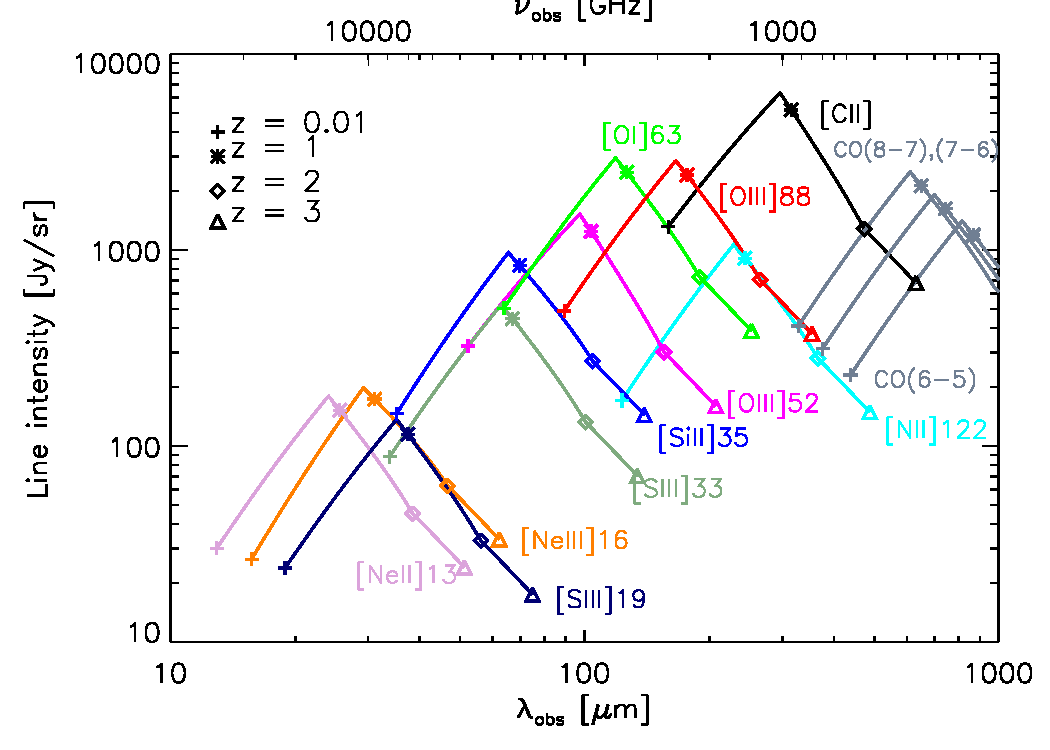
\includegraphics[width=0.4\textwidth]{interloper_intensity_jysr}
\caption{Intensity of fine structure line emission as a function of observed wavelength for the empirical model based on the B11 luminosity function.}
\label{fig:interlopers}
\end{figure}

The resulting mean intensities for a variety of FIR lines are plotted in Figure~\ref{fig:interlopers} as a function of redshift and observed wavelength. $\bar{S}_{i}$ vs $\lambda_{obs}$ can be interpreted as identifying the dominant source of fluctuations, according to our model, for a given frequency. As a specific example, if the target line of an observation is [OI]63$\mu$m at $z = 1$, it is necessary to distinguish between the target line and interlopers from different redshifts which nonetheless contribute power at the observed frequency. Visbal and Loeb (2010) showed how the cross spectra can be used to differentiate between a target line and a contaminating line (or ``bad line", in their words), since emitters at different redshifts will be spatially uncorrelated. For the observed wavelengths of [CII], however, it is apparent from Figure 2 that, with the exception of contributions from [OIII]88$\mu$m near $z \sim 0.01$, the [CII] line is not vulnerable to confusion with interlopers.  

%\begin{equation}
%P_{i,j}(k,z)& = \bar{S}_i(z) \bar{S}_j(z) \bar{b}_i(z) \bar{b}_j(z) P_{nl}(k,z) + P_{shot}^{i,j}(k) %\\
%\end{equation}

%In the case of far-IR lines, where there is no observational evidence of emitting populations with distinct clustering properties, it is justified to take $\bar{b}_i(z) = \bar{b}_j(z)$. Note that this equality may not hold between the far-IR lines and certain near- and mid-IR lines, which are primarily produced in AGN, and which may have different clustering characteristics.

%Incorporating the IR luminosity function in the approach to estimating the [CII] density facilitates the separation of [CII]-emitting galaxies by luminosity class, i.e., ULIRG, LIRG, or normal galaxy, which is useful since there is not a one-to-one mapping of [CII] luminosity to infrared luminosity for individual galaxies. To understand, then, the relation between [CII] emission from a diverse ensemble of galaxies present in the power spectrum to the star formation rate at a given redshift, it is imperative to sort out the mix of galaxy types and corresponding luminosities that contribute to the total emission. We use the recent compilation of Gracia-Carpio et al. (2011) for the measured relation of $L_{[CII]}$ to $L_{FIR}$ in a range of systems. 

%For most normal galaxies (here taken to mean $L_{FIR} < 10^{11} L_{\odot}$) at any redshift, the $L_{[CII]}/L_{FIR}$ ratio is approximately equal to $3 \times 10^{-3}$ (with a $1-\sigma$ scatter of only $\sim$ 0.3 dex). Since $L_{FIR}$ is well known to tightly correlate with SFR (Kennicutt??), for these systems the $L_{[CII]}$ traces the SFR with a known proportionality constant. 

%In the local universe, dense, high ionization environments are typical of the central star-forming regions of ULIRGs ($L > 10^{12} L_{\odot}$) or LIRGS ($L>10^{11} L_{\odot}$). These environments exhibit underluminous [CII] emission because [CII] is strongly sensitive to the intensity of the UV field and saturates at high UV fluxes. For nearby sources with $L>10^{12} L_{\odot}$, $L_{[CII]}/L_{FIR}$ drops by a factor of $\sim$ 5-10, and $L_{[CII]}$ no longer scales with SFR, but such sources are rare at $z<0.01$ and account for only a small fraction of the total SFR density. Hence, at these redshifts, the bulk of the [CII] emission is from "normal"-type galaxies that obey the relatively tight correlation between $L_{[CII]}-L_{FIR}$. 

%By contrast, at $z \sim 1$, the fraction of SFRD contributed by high luminosity sources substantially increases. At $z = 1-2$, however, the Stacey et al (2010) results show that the threshold for a significant deficiency in $L_{[CII]}$ rises to $L \sim 5 \times 10^{12} L_{\odot}$ (Figure ??), so that the majority of the emission again still adheres to a relatively tight correlation, and the fraction contributed by sources with weak [CII] appears to remain negligible at all redshifts. 

%We can characterize the redshift evolution of $\kappa$ from the IR luminosity function. This behavior is plotted in Figure XXX. 


%\begin{equation}
%\bar{L}_{\mathrm{[CII]}} = \int_{L_{IR}^{min}}^{L_{IR}^{max}} \! \mathrm{d}(\mathrm{log_{10}} \, L_{IR}) L_{IR} \Phi(L_{IR}, z) f_{[CII]}(L_{IR}).
%\end{equation}

%The fraction $f_{[CII]}(L_{IR})$ is obtained from the fit for [CII] luminosity---based on local ISO-LWS observations (Brauher et al 2008)---as a function of IR luminosity provided by Spinoglio et al (2011, their equation 33, reproduced below):

%\begin{equation}
%\begin{split}
%f_{[CII]}(L_{IR})& =\frac{L_{[CII]}}{L_{IR}}\\
%                           & =\frac{(0.89 \pm 0.03) \mathrm{log_{10}}L_{IR} - (2.44 \pm 0.07)}{L_{IR}}.
%\end{split}
%\end{equation}

%Finally, in terms of the IR luminosity function, the shot noise becomes

%\begin{multline}
%P_{shot}^{\mathrm{[CII],[CII]}}(k) =  \int_{L_{IR}^{min}}^{L_{IR}^{max}} \! \mathrm{d}(\mathrm{log_{10}}L_{IR}) \, \Phi(L_{IR}, z)\\
%\times  f_{[CII]}(L_{IR}) \left( \frac{L_{\mathrm{[CII]}}}{4\pi D_L^2} \right)^2 \left( \frac{\mathrm{d}\chi}{\mathrm{d}\nu} D_A^2 \right)^2
%\end{multline}

%It should be noted that the mean [CII] luminosity $\bar{L}^{[CII]}$ does, in reality, include a contribution from diffuse gas in the intergalactic medium (IGM), yet Gong et al (2012) estimated that the specific intensity coming from the IGM ranges from $\sim 10^{-3}$ Jy sr$^{-1}$ to $\sim$ 1 Jy sr$^{-1}$ at $z = 1$---a negligible amount compared to the emission from the interstellar medium (ISM) of galaxies. 

\section{The [CII] Power Spectrum}

\subsection{Sensitivity forecast}

We present in this section predictions for the [CII] power spectrum with error bar estimates for a feasible experimental platform, namely, a balloon-borne experiment that allows for uninterrupted spectral coverage in the wavelength range 240 to 420 $\mu$m pertinent to this study. Fiducial experimental parameters are summarized in Table ~\ref{tab:ExpParams}. The telescope mirror aperture, $D_{ap}$, survey area, $A_{survey}$, and total observing time, $t_{obs}^{survey}$, are taken as 2.5 m, 1 deg$^2$, and 200 hours, respectively, though we explore the effect of varying $D_{ap}$ and $A_{survey}$ on SNR (cf. Figure~\ref{fig:snr_nmode_k}).

Predictions for the fiducial case---as computed from the method of combining the cosmological matter power spectrum and the IR LF model outlined in Section 2.1---for the  [CII] power spectrum at four redshifts $z = 0.63, 0.88, 1.16$, and $1.48$ are shown in Figure~\ref{fig:pcii_zall}. (Note that we use  $\Delta_{[CII],[CII]}^2 = k^3 P_{[CII], [CII]}(k)/(2\pi^2)$ when plotting the power spectrum. In this notation, the factor $k^3$ cancels out the volumetric units of $P_{\delta,\delta}(k,z)$ and the integral of $\Delta_{[CII],[CII]}^2$ over logarithmic k bins is equal to the variance in real space.) At these redshifts, respectively, the average linear bias has been assumed to be $\bar{b} = 2.0, 2.3, 2.6$, and $2.9$, in line with theoretical predictions from (Cooray and Sheth ???). The crossing of the one-halo and two-halo terms in the power spectrum can be detected with SNR of order 10 at all redshifts.  In calculating the power spectrum sensitivity, the two lowest line-of-sight modes and the lowest transverse mode are not included, since these modes will likely be compromised by the necessity of continuum foreground subtraction and beam-differencing in the fluctuation analysis. The exact effect of continuum subtraction will need to be modeled via simulation. 

Error bar estimates and the total SNR for the power spectrum are calculated by assuming a spectrally flat noise power spectrum, so that the noise power in each pixel, $P_{N}$, is written as

\begin{equation}
P_N = \sigma_N^2 \frac{V_{pix}}{t_{pix}},
\end{equation}

where $\sigma_N^2$ is the instrument sensitivity (noise equivalent intensity, or NEI, in units of Jy sr$^{-1}$ s$^{1/2}$, $V_{pix}$ is the volume of a pixel, and $t_{obs}^{pix}$ is the time spent observing on a single pixel. The variance of a measured $k$, $\sigma^2(k)$, is then written as

\begin{equation}
\sigma^2(k) = \frac{\left({P_{[CII],[CII]}(k) + P_N(k)}\right)^{2}}{N_{modes}},
\end{equation}

where $N_{modes}$ is the number of wavemodes that are sampled for a given $k$ bin of some finite width $\Delta$log(k). (We have chosen $\Delta$log(k) = 0.3 for this analysis.)

The total SNR, in turn, is calculated from the expression 

\begin{equation}
SNR_{tot} = \sqrt{\sum_{bins} \left(\frac{P_{[CII],[CII]}(k)}{\sigma(k)}\right)^2}
\end{equation}

Note that it is possible to rewrite $P_N$ in terms of the parameters from Table 1, giving 

\begin{equation}
\begin{split}
P_N& = \left(\sigma_N^2 A_{pix} \Delta r_{los}^{pix}\right) / \left({\frac{t_{survey}}{n_{beams}/N_{instr}^{spatial}}}\right) \\
& = \left(\sigma_N^2 A_{pix}\Delta r_{los}^{pix}\right) /  \left(\frac{t_{survey} N_{instr}^{spatial}}{A_{survey}/A_{pix}}\right)\\
& = \sigma_N^2 \frac{\Delta r_{los}^{pix} A_{survey}}{t_{survey} N_{instr}^{spatial}}
\end{split}
\label{eq:pnoise}
\end{equation}

In this form, it becomes apparent that---with fixed number of spatial pixels, spectral resolution, and total observing time---the only factor driving up the amplitude of noise power is the survey area; the effect of increasing aperture only allows access to higher wavenumbers, which can be useful for subtracting the shot noise from the total power in later steps of data analysis.This behavior is shown clearly in Figure 5, where the SNR is plotted as a function of $k$ for different survey geometries and both mirror diameters.

\begin {table*}[h]
\begin{center}
\caption {Fiducial Parameters for Envisioned Balloon Experiment} \label{tab:ExpParams} 
\begin{tabular}{ l c c c c}
\hline \hline
$R = \nu_{obs} / \delta\nu$ & \multicolumn{4}{c}{450} \\
  $t_{obs}^{survey}$ (hr)&\multicolumn{4}{c}{200}\\
  $D_{ap}$ (m) &\multicolumn{4}{c}{2.5}\\
$A_{survey}$ (deg$^2$) &\multicolumn{4}{c}{1.0}\\
\hline
 $z$ & 0.63 & 0.88 & 1.16 & 1.48 \\
 $\bar{S}_{[CII]}$ (Jy sr$^{-1}$) & 4.56 $\times 10^3$ & 6.33 $\times$ 10$^3$ & 4.05 $\times 10^3$ & 2.55 $\times 10^3$ \\
 NEI (10$^7$ Jy sr$^{-1}$ sec$^{1/2}$) & 3.4 & 2.1 & 1.5 & 1.0 \\
 Line Sensitivity (10$^{-17}$ W m$^{-2}$ sec$^{1/2}$) & 1.58 & 1.13 & 0.92 & 0.71 \\
 Wavelength Range ($\mu$m) & 240-276 & 276-317 & 317-365 & 365 - 420\\
 $\delta\nu$ (GHz) & 2.58 & 2.25 & 1.95 & 1.70 \\
 \hline
 \end{tabular}
 \end{center}
 \end{table*}
 %\hline
 % $A_{s}$ (deg$^2$)&\multicolumn{3}{c}{1.0}&\multicolumn{3}{c}{5.3}&\multicolumn{3}{c}{10.0}&\multicolumn{3}{c}{1.0}&\multicolumn{3}{c}{5.3}&\multicolumn{3}{c}{10.0}\\
%  $V_{s}$ (Mpc$^3$ h$^{-3}$)&\multicolumn{3}{c}{6.90 $\times 10^5$}&\multicolumn{3}{c}{3.66 $\times 10^6$}&\multicolumn{3}{c}{6.89 $\times 10^6$}&\multicolumn{3}{c}{1.40 $\times 10^6$}&\multicolumn{3}{c}{7.42 $\times 10^6$}&\multicolumn{3}{c}{1.40 $\times10^7$}\\
%  $P_{N}$ ($10^{11}$Jy$^2$ sr$^{-2}$ Mpc$^3$ h$^{-3}$)&\multicolumn{3}{c}{2.64}&\multicolumn{3}{c}{140}&\multicolumn{3}{c}{264}&\multicolumn{3}{c}{1.22}&\multicolumn{3}{c}{6.44}&\multicolumn{3}{c}{121}\\
%  \hline
 % $D_{ap}$ (m) & 0.8 & 2.5 & 8.0 & 0.8 & 2.5 & 8.0 & 0.8 & 2.5 & 8.0 & 0.8 & 2.5 &8.0 & 0.8 & 2.5 & 8.0 & 0.8 & 2.5 & 8.0 \\
 % Beam FWHM (arcmin) & 0.16 & 0.50 & 1.6 & 0.16 & 0.50 & 1.6 & 0.16 & 0.50 & 1.6 & 0.16 & 0.50 & 1.6 & 0.16 & 0.50 & 1.6 & 0.16 & 0.50 & 1.6 \\
 % $t_{pix}$ (hr) & 0.0345 & 0.345 & 3.45 & 0.00651 & 0.0651 & 0.651 & 0.00345 & 0.0345 & 0.345 & 0.0604 & 0.604 & 6.04 & 0.0114 & 0.114 & 1.14 & 0.00604 & 0.0604 & 0.604 \\
%  $SNR_{tot}$ & 35 & 20 & 15 & 16 & 10 & 8.4 & 12 & 7.8 & 6.5 & 48 & 19 & 10.1 & 21 & 8.5 & 4.9 & 16 & 6.3 & 3.8 \\
 % $SNR_{tot}^{clust}$ & 14 & 14 & 15 & 7.8 & 7.8 & 7.6 & 6.1 & 6.1 & 6.1 & 7.1 & 7.3 & 6.9 & 3.7 & 3.7 & 3.6 & 2.8 & 2.9 & 2.9 \\
 % \hline
%\end{tabular}
%\end{center}
%\end{table}
%\end{sidewaystable*}

\begin{figure}[h]
\centering
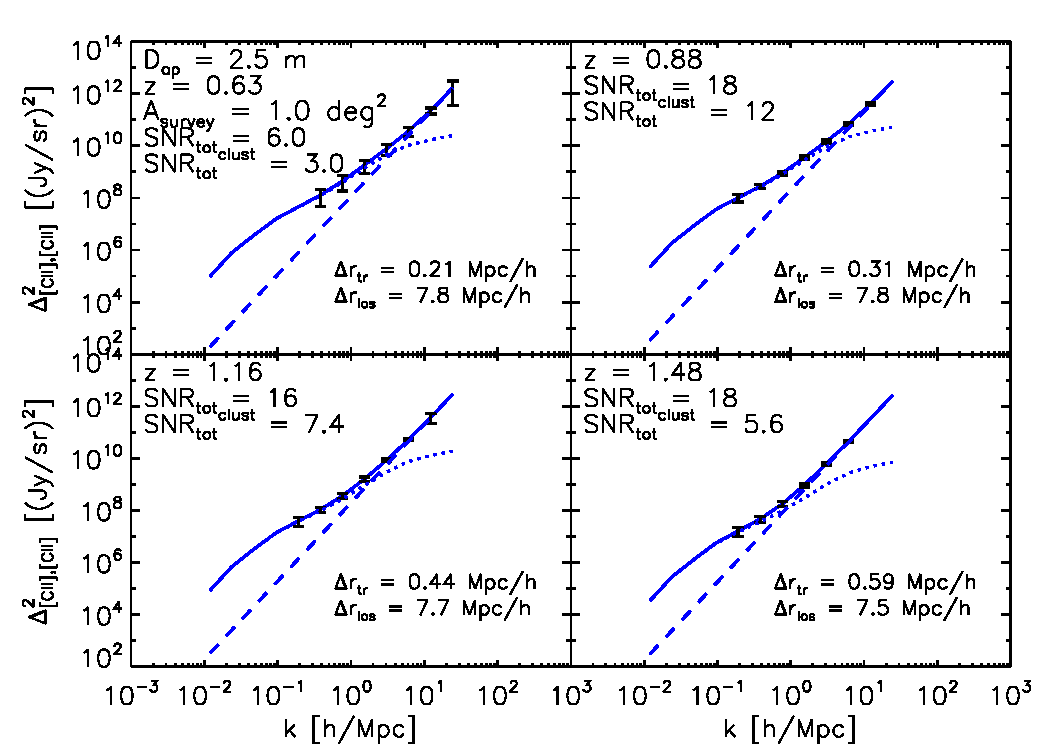
\includegraphics[width = 0.5\textwidth]{pcii_STARFIRE_z63_z88_z116_z148_halofit_bethermin_spinoglio_ap2p5m_1sqdeg_uhp_ktnonzero}
\caption{Predicted [CII] power spectra with error bar estimates from $z$ = 0.63 to $z$ = 1.48 for telescope with 2.5 meter aperture and a survey area of 1 square degree. Dotted curves indicate power from clustering (including contributions from linear and nonlinear terms), and dashed curves indicate the contribution from shot noise power.}
\label{fig:pcii_zall}
\end{figure}

\begin{figure}[h]
\centering
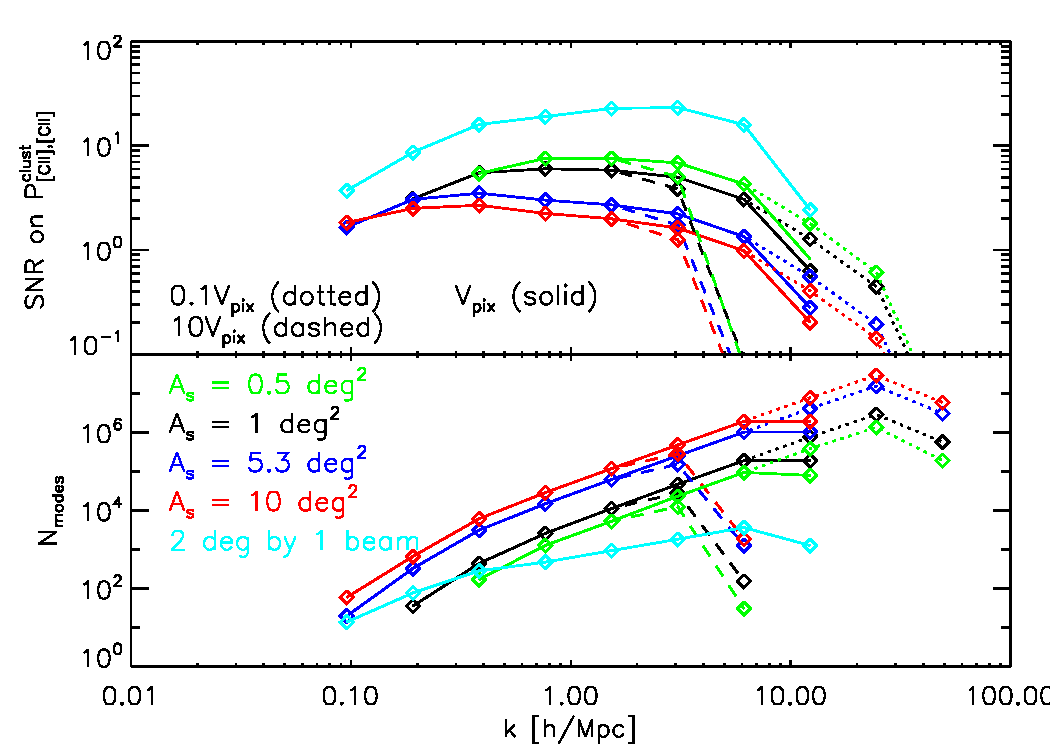
\includegraphics[width=0.5\textwidth]{snr_nmode_vs_k_starfire_ap2p5m_0p1vpix_10vpix_1sqdeg_5p3sqdeg_10sqdeg_ktnonzero}
\caption{Signal-to-noise on the clustering term of the [CII] power spectrum $P_{\textrm{[CII], [CII]}^{clust}}$ and number of modes as a function of $k$ at $z=0.88$. The black, blue, and red lines correspond to survey areas of 1.0, 5.3, and 10.0 deg$^2$, respectively. Telescopes with apertures yielding 0.1, 1, and 10 times the fiducial pixel volume, $V_{pix}$, are shown as the dotted, solid, and dashed lines, respectively.}
\label{fig:snr_nmode_k}
\end{figure}

\subsection{Measuring $\bar{S}_{[CII]}(z)$}

Recall that the [CII] clustering power spectrum, $P_{\textrm{[CII],[CII]}}^{clust}$, as measured by intensity mapping is sensitive to intensity fluctuations from the full range of normal to ULIRG-class systems because its amplitude is proportional to the mean line intensity, squared. The effect on the measured power spectrum of limiting the galaxy populations (categorized by their IR luminosities) that are observed in the fiducial survey field is depicted in Figure~\ref{fig:pcii_lirmin}. In this Figure, we see the clustering amplitude decrease as the IR detection threshold, $L_{IR, min}$, is raised from 10$^{8}$ L$_{\odot}$ to 10$^{12}$ L$_{\odot}$.  The reduction in the clustering amplitude is quantified in Figure~\ref{fig:frac_cii_b11_lirmin}, which shows how the observed signal---expressed in terms of the observed fraction of $\bar{S}_{\textrm{[CII]}}$---depends on $L_{IR,min}$ for our empirically-based model.

The level of decrease in clustering power as a result of raising $L_{IR,min}$ is most dramatic at the lower end of the redshift range of interest, when the luminosity function is represented mostly by normal galaxies and LIRGs. As ULIRGs rise to dominate the IR luminosity density at $z \sim 1.5$, we see that SNR on the power spectrum becomes relatively robust until $L_{IR,min} =$ 10$^{12}$ L$_{\odot}$. In fact, we infer from Figure~\ref{fig:frac_cii_b11_lirmin} that at $z = 1.48$, that individually resolving galaxies at a depth of $6\times10^{11}$ L$_{\odot}$ will recover half of $\bar{S}_{\textrm{[CII]}}$. (For redshifts $z = 0.63, 1.16, and 3.0$, the corresponding depths to observe half of the [CII] light are $\sim 10^{11}$, $2\times10^{11}$, and $10^{12}$ L$_{\odot}$, respectively.)

\begin{figure}
\centering
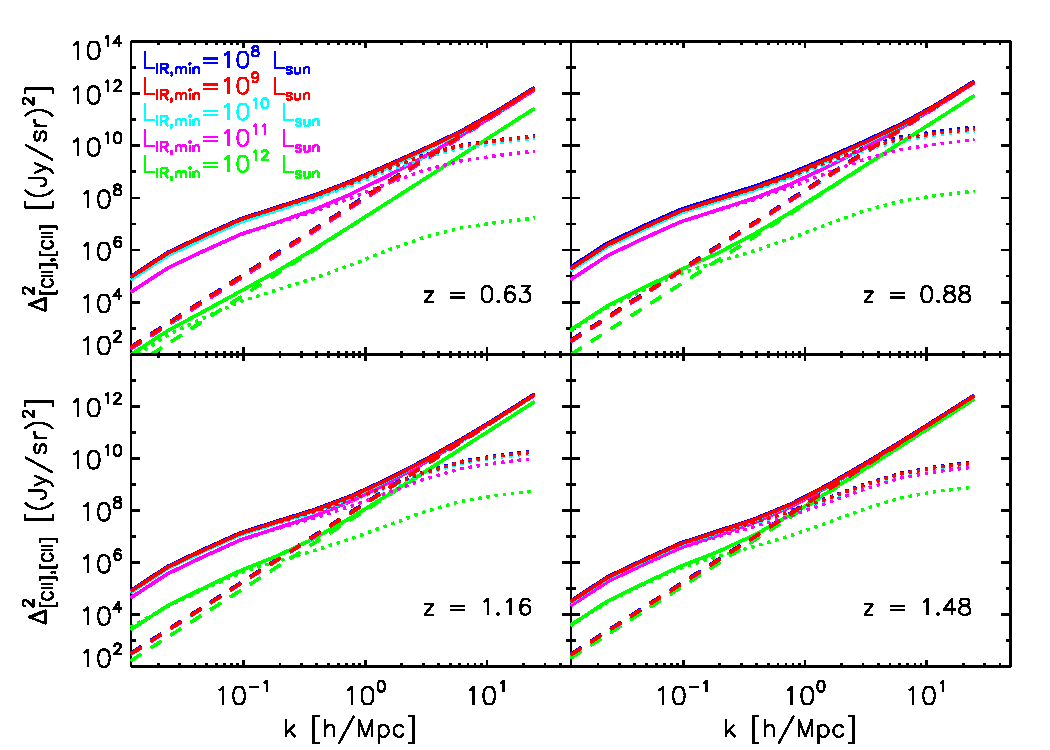
\includegraphics[width=0.5\textwidth]{pcii_STARFIRE_z63_z88_z116_z148_lirmin_halofit_bethermin_spinoglio_ap2p5m_1sqdeg_uhp_ktnonzero}
\caption{Predicted [CII] power spectra from $z = 0.63$ to $z = 1.48$. Blue, red, cyan, magenta, and green curves represent the power spectrum computed with a lower limit in the luminosity function corresponding to $10^8$, $10^9$, $10^{10}$, $10^{11}$, and $10^{12}$ L$_{\odot}$, respectively.}
\label{fig:pcii_lirmin}
\end{figure}

\begin{figure}
\centering
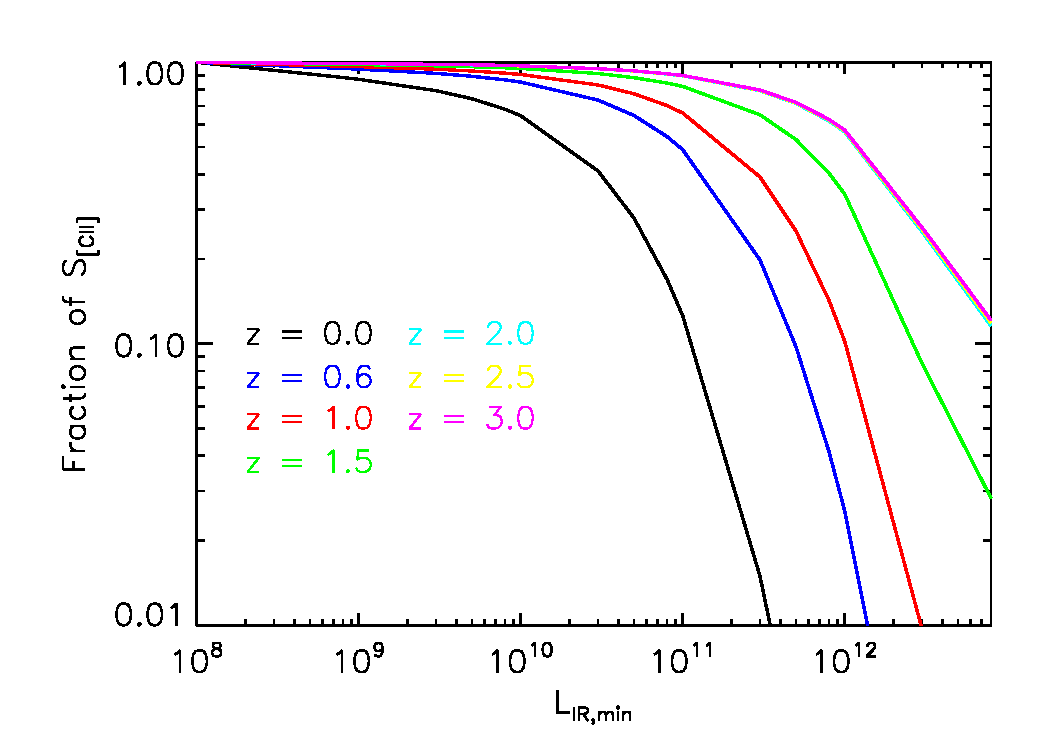
\includegraphics[width=0.5\textwidth]{fraction_cii_emissivity_vs_LIRmin_vs_z}
\caption{The fraction of total [CII] mean intensity as a function of lower limit in the luminosity function. Different color curves represent different redshifts, as labeled on the plot.}
\label{fig:frac_cii_b11_lirmin}
\end{figure}

To avoid missing the fainter systems when quantifying the mean [CII] intensity, and thus ensure a complete view of the extragalactic [CII]-emitting populations, we introduce intensity mapping as a means of measuring $\bar{S}_{\textrm{[CII]}}$ and its evolution across cosmic time. In order to successfully extract $\bar{S}_{\textrm{[CII]}}$ from the power spectrum, then, it is necessary to divide out $P_{\delta,\delta}(k,z)$ and $\bar{b}_{\textrm{[CII]}}^2(z)$. (High sensitivity on shot noise-dominated modes ensures that the preliminary step of accurate shot noise subtraction is readily attainable.) The confidence with which these are \emph{a priori} known quantities becomes lower as $k$ increases. For example, the 1-halo power spectrum for DSFGs appears to be dependent on $L_{IR}$ of the contributing sources (Viero et al 2013), indicating the need to map sufficiently wide areas that access $k$ modes where the power is largely independent of the level of 1-halo power. 

Returning to Figure~\ref{fig:snr_nmode_k}, we see that, for the purpose of measuring $\bar{S}_{\textrm{[CII]}}$ with the fiducial survey of 1 deg$^2$, there are two $k$ bins, namely, $k = 0.16$ and 0.27 h/Mpc in which the 2-halo clustering accounts for at least 75\% of the total power. (Surveys with $A_{survey} = 5.3 and 10$ deg$^2$, also shown in Figure~\ref{fig:snr_nmode_k}, are wide enough to have three $k$ bins available in the linear regime, but the sensitivity on the additional mode with $t_{obs}^{survey}$= 200 hours is marginal.) Thus, in considering the case of $A_{survey} = 1.0$ deg$^2$, we find that it is possible to measure $\bar{S}_{\textrm{[CII]}}(z)$ within $\sim10\%$ accuracy from $z = 0.63$ to $z=1.48$, as shown in Figure~\ref{fig:scii_z}, where the fractional uncertainty on $\bar{S}_{\textrm{[CII]}}(k,z)$ has been calculated as half the fractional uncertainty on $P_{\textrm{[CII],[CII]}}(k,z)$.

\begin{figure}[!h]
\centering
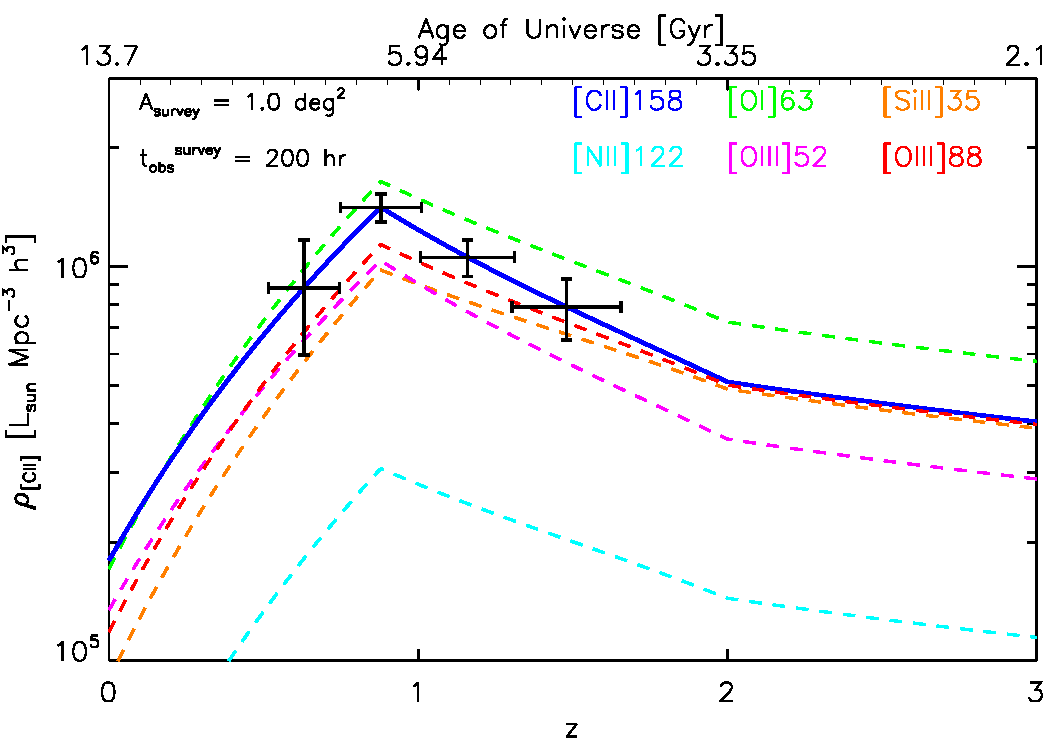
\includegraphics[width=0.5\textwidth]{rhocii_vs_z_starfire_1sqdeg_tobs200hr}
\caption{Error bar estimates on $\rho_{[CII]}$, as measured by the fiducial experiment, at observed redshifts $z$ = 0.63, 0.88, 1.16, and 1.48. Errors in $z$ correspond to the redshift space spanned by the spectrometer bandwidth. The solid blue curve is the underlying model for [CII] mean intensity. The luminosity density of other bright IR lines are shown as the dashed colored curves.}
\label{fig:scii_z}
\end{figure}

\section{Observational Strategy}

Now let us turn to a question regarding the motivation for intensity mapping in general, as well as in the specific case of [CII] at the redshifts relevant to this study. Having identified the galaxy redshift surveys as an alternative method to measure the 3D clustering power spectrum, it is natural to ask: In which regime does intensity mapping measure the power spectrum with higher SNR than the traditional galaxy surveys?

The expressions for SNR on a $k$ bin of interest for galaxy and intensity mapping surveys (denoted, respectively, by the subscripts ``GS" and ``IM") are

\begin{eqnarray}
\textrm{SNR}_{GS}  = \frac{\sqrt{N_{modes}} }{1 + 1/(b_i^2P_{\delta,\delta}\bar{n}_{gal} )} \\
\textrm{SNR}_{IM} =  \frac{\sqrt{N_{modes}}}{1 + P_N/\left(\bar{S}_{i}^2b_i^2P_{\delta,\delta}\right)}
\end{eqnarray}

To facilitate our comparisons in what follows, we employ toy models for the IR LF (Figure ~\ref{fig:schechterfuncs}) written in the Schechter formalism---parametrized by the usual $\alpha$, $L_*$, and $\phi_*$---and normalize the total luminosity density to the empirical model from Section 2 (cf. Appendix for details). We stress that these Schechter models are not intended to represent a real interpretation of the distribution of galaxies, but are merely helpful for illustrating the effect of the LF \emph{shape} on the relative usefulness of intensity mapping and traditional galaxy surveys.

\begin{figure}
\centering
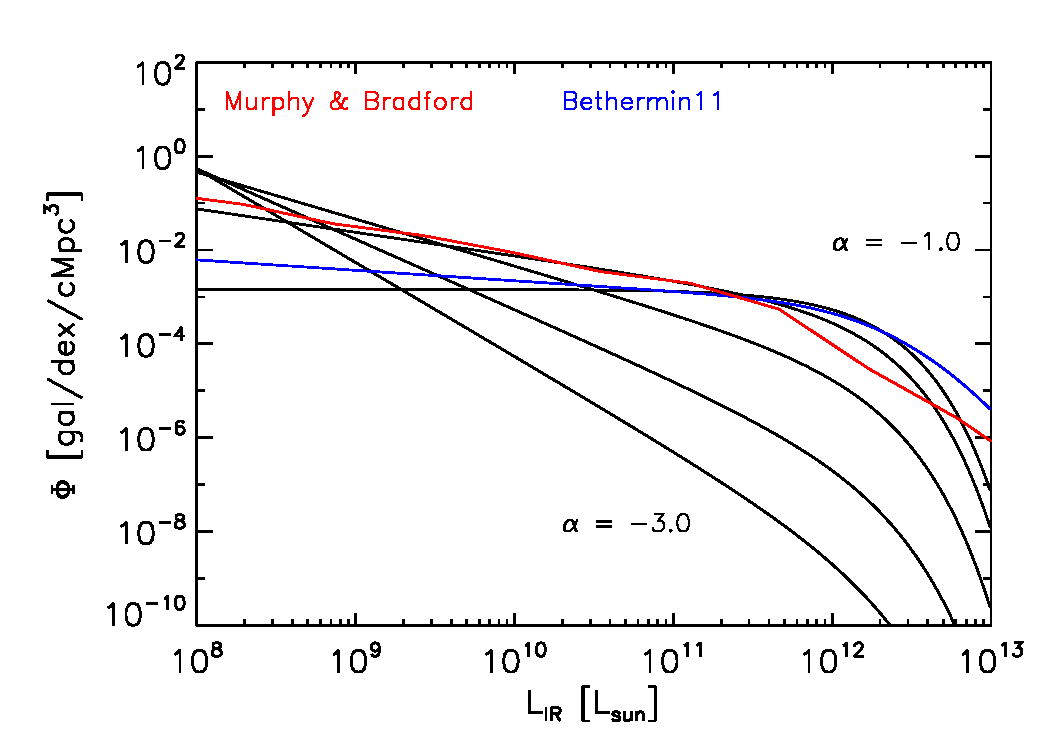
\includegraphics[width=0.5\textwidth]{phi_lir_schechter_bethermin11_murphy_Lstar1d12_Lmin1d8_Lmax1d13}
\caption{Toy model IR luminosity functions with faint-end slope (from top to bottom) $\alpha=-1.0, -1.5, -2.0, -2.5, -3.0$. The B11 and Muprhy \& Bradford models are plotted as blue and red curves, respectively, for comparison.}
\label{fig:schechterfuncs}

\end{figure}

The line sensitivity, $S_{\gamma}$ (units of W m$^{-2}$ s$^{1/2}$), is the figure of merit for detecting an unresolved line in a point source, and we define individual detections at the $5\sigma$ level as having a flux above the instrumental noise in a pixel, i.e., above $5 \times S_{\gamma} t_{pix}^{-1/2}$. (For this analysis, we have assumed the galaxy surveys have reliable spectroscopic redshifts and thus neglect the problem of confusion noise.) %A convenient expression, which explicitly ties the minimum detectable luminosity to a broader framework of experimental variables, for the detection threshold can be written as
%\begin{equation}
%L_{i, min} = 5 \times f_{err}\rho_i V_{pix}, 
%\end{equation}
%Here, $f_{err}$ is the fractional error, 
%\begin{equation}
%f_{err} = \left(\frac{\sigma_N}{\sqrt{t_{pix}}}\right)/\bar{S}_i(z)
%\end{equation}
% and $\rho_{i}(z)$ is the comoving luminosity density of line $i$ at some $z$, or $L_*\phi_* \Gamma(2+\alpha, L/L_*)$ in the Schechter notation, so that
%\begin{equation}
%\frac{L_{i,min}}{4\pi D_L^2} \Leftrightarrow 5 \times S_{\gamma} t_{pix}^{-1/2}
%\end{equation}
 
%Recall that the units of $\frac{\sigma_{N}}{\sqrt{t_{pix}}}$ and $S_{i}$ are Jy sr$^{-1}$, which does not depend on aperture. One converts between $\sigma_N$ and $S_{\gamma}$ by dividing (or multiplying) by the frequency resolution d$\nu$ and beam solid angle d$\Omega$.
 
Since the intensity mapping technique contains information in the power spectrum from sources below a given $S_{\gamma}$, we expect that regimes in which the majority of galaxies are too faint to be resolved are better-suited for intensity mapping observations than observations via the traditional galaxy survey. 

One such regime is when the bulk of the galaxy number density at a certain redshift is comprised of galaxies with sub-$L_*$ luminosities (i.e., for steep slope $\alpha$ in the LF). Indeed, this case is illustrated in the middle and righthand panels of Figure~\ref{fig:snr_vs_time_z1p5}, where, for LFs with $\alpha < -1.5$, the intensity mapping method (magenta curve) has higher SNR than the corresponding galaxy survey performed with the same instrument (dashed black curve), for all survey observing times. (Note the galaxy survey and intensity mapping survey map the same fiducial area in this example.) However, for the flattest faint-end slope ($\alpha = -1$, lefthand panel), both techniques have comparable SNR for most observing times. We point out that SNR$_{IM} >$ SNR$_{GS}$ for very short and very long observing times, which correspond to shot-noise dominated and cosmic variance-dominated regimes, respectively, for the galaxy surveys. 

Figure~\ref{fig:snr_vs_time_z1p5} also shows the effect of changing pixel area by a factor $\epsilon$---due to a change in the telescope's aperture diameter by $\epsilon^{-1/2}$---on the SNR. Because the area of the survey is fixed, the transformation on pixel area leads to a change in $S_{\gamma}$ by the same factor $\epsilon$, but will not alter $P_{N}$ (as seen previously in Eq.~\ref{eq:pnoise}) for the intensity mapping experiment; SNR$_{IM}$ is robust to changes in pixel area. Thus, the instruments with smaller pixels (triple-dot dashed curve, $\epsilon = 0.1$) achieve greater depths than their large pixel counterparts (dot-dashed curve, $\epsilon = 10.0$), and thus attain higher SNR by resolving more galaxies. Meanwhile, galaxy surveys with large pixels find themselves in the disabling condition of having many sources that are below the detection threshold in a single voxel. Whether or not the galaxy survey experiments with small pixel area outperform the intensity mapping experiment is, however, dependent on the faint-end slope of the luminosity function. 
 
 
 
%V_{pix}$ suggests that traditional galaxy surveys with large voxels, such that $L_*\phi_* \Gamma(2+\alpha, L/L_*) V_{pix} \gg 1$, will find themselves in the disabling condition of having many sources that are below the detection threshold in a single voxel. On the other hand, because the intensity mapping method does not aim to detect individual galaxies, it will still be able to measure clustering in the large voxel limit with high SNR.  We juxtapose in Figure \ref{fig:snr_vs_time_z1p5} the SNR for the fiducial intensity mapping experiment and galaxy surveys in both the large and small pixel limit in the context of our example for the [CII] power spectrum at $z = 1.48$. As seen in the previous section, a change in aperture does not affect the SNR$_{IM}$ for $k < 0.1$ h/Mpc, but, as expected, dramatically enhances or degrades the capability of galaxy surveys in measuring the power spectrum.  From Figure \ref{fig:snr_vs_time_z1p5} it is clear that the fiducial intensity mapping experiment outperforms galaxy surveys at $z=1.48$ for luminosity functions with faint-end slope $\alpha$ of the tested luminosity functions, and, that this disparity is enhanced in the large pixel limit. In the small pixel limit however, where we expect the galaxy surveys to be capable of measuring the power spectrum with high significance, we see that it becomes important to consider the shape of the luminosity function when drawing conclusions about whether to intensity map or perform a traditional galaxy survey. In fact, it seems that only for the flattest luminosity functions does the small pixel limit improve SNR$_{tot, GS}$ such that it becomes higher than SNR$_{tot,GS}$.

 
 %\begin{figure}
%\centering
%\includegraphics[width=0.5\textwidth]{lirmin_lsun_tsurvey_z1p5_1sqdeg_0p1vpix_vpix_10vpix}
%\caption{$L_{IR,min}$ as a function of the survey observing time, for the various $V_{pix}$, at $z = 1.5$. The value of our adopted $L_{*}$ is plotted for comparison.}
% \label{fig:lirmin_z1p5}
%\end{figure}

%Written in this way, the expression for the detection threshold $L_{i,min}$ already provides some insight as to the optimal regimes for intensity mapping and galaxy surveys. Firstly, for $L_{i,min} \ll L_*$, we expect the galaxy surveys to be an effective means of studying the galaxy population, since the number of detections will be high and the shot noise term will be low. Conversely, if $L_{i, min} \gg L_*$, then the galaxy survey will not be able to detect a significant fraction of galaxies that comprise the faint-end of the luminosity function, and intensity mapping becomes the ideal survey method, since it is sensitive to the total emission at a given redshift.

%Now, suppose the voxels are changed in size by some factor $\epsilon$ due to a change in aperture diameter by $\sqrt{\epsilon}$, but the survey area and survey observing time are left the same, leading to the following transformations on $t_{pix}$, the large scale clustering modes $N_{modes}^{clust}$, $P_{N}$, $f_{err}$, and, ultimately, $L_{i,min}$:

%\begin{eqnarray}
%t_{pix} \rightarrow t_{pix}^{\prime} &= \epsilon t_{pix} \\
%N_{modes}^{clust} \rightarrow N_{modes}^{clust \prime} &= N_{modes}^{clust} \\
%P_N \rightarrow P_N^{\prime} &= P_{N} \\
%f_{err} \rightarrow f_{err}^{\prime} &= \frac{f_{err}}{\sqrt{\epsilon}} \\
%L_{i,min} \rightarrow L_{i,min}^{\prime} &= \sqrt{\epsilon} L_{i,min}
%\end{eqnarray}

%We take a moment to point out that an increase in aperture diameter by $\sqrt{\epsilon}$ also results in an increase in the righthand side of Equation 15 by the same factor $\sqrt{\epsilon}$ that appears in Equation 20 after applying the analogous transformations for the line sensitivity:

%\begin{eqnarray}
%S_{\gamma} \rightarrow S_{\gamma}^{\prime} = \epsilon S_{\gamma}\\
%t_{pix} \rightarrow t_{pix}^{\prime} = \epsilon t_{pix} \\
%\end{eqnarray}

%Thus, the increase of $L_{i,min}$ with $V_{pix}$ suggests that traditional galaxy surveys with large voxels, such that $L_*\phi_* \Gamma(2+\alpha, L/L_*) V_{pix} \gg 1$, will find themselves in the disabling condition of having many sources that are below the detection threshold in a single voxel. On the other hand, because the intensity mapping method does not aim to detect individual galaxies, it will still be able to measure clustering in the large voxel limit with high SNR.  We juxtapose in Figure \ref{fig:snr_vs_time_z1p5} the SNR for the fiducial intensity mapping experiment and galaxy surveys in both the large and small pixel limit in the context of our example for the [CII] power spectrum at $z = 1.48$. As seen in the previous section, a change in aperture does not affect the SNR$_{IM}$ for $k < 0.1$ h/Mpc, but, as expected, dramatically enhances or degrades the capability of galaxy surveys in measuring the power spectrum.  From Figure \ref{fig:snr_vs_time_z1p5} it is clear that the fiducial intensity mapping experiment outperforms galaxy surveys at $z=1.48$ for luminosity functions with faint-end slope $\alpha$ of the tested luminosity functions, and, that this disparity is enhanced in the large pixel limit. In the small pixel limit however, where we expect the galaxy surveys to be capable of measuring the power spectrum with high significance, we see that it becomes important to consider the shape of the luminosity function when drawing conclusions about whether to intensity map or perform a traditional galaxy survey. In fact, it seems that only for the flattest luminosity functions does the small pixel limit improve SNR$_{tot, GS}$ such that it becomes higher than SNR$_{tot,GS}$.

In Figure ~\ref{fig:ngal_frac}, SNR$_{GS}$  is broken down in terms of the number of 5$\sigma$ detections (left panel) and the observed [CII] luminosity density, $\rho_{[CII], obs}$, relative to the total [CII] luminosity density, $\rho_{[CII]}$ (right panel). While it is possible to reach SNR$_{GS} \sim 10$ with $\sim 100$ galaxies in 200 hours with the fiducial instrument and survey area, the actual fraction of [CII] emission supplied by these detected galaxies is close to 20\%. To recover 50\% or greater of $\rho_{[CII]}$, one must observe for longer than several thousand hours. (For LFs with slopes steeper than $\alpha = -1.0$, the required observing times are significantly longer due to the larger population of faint galaxies.) If, however, one extracts the aggregate, unresolved emission from [CII] via the intensity mapped power spectrum, one is essentially measuring $\frac{\rho_{[CII], obs]}}{\rho_{[CII]}} = 1$ as soon as SNR$_{IM}$ on the linear clustering term of the power spectrum is sufficiently high, which we depict in Figure~\ref{fig:scii_z} for a 5.3 deg$^2$ survey with $t_{obs}^{survey} = 1,000$ hr.



%Another scenario in which an experiment finds itself in the large pixel limit is for observations at long wavelengths. Figure ~\ref{fig:snr_vs_time_z6} shows the envisioned balloon-borne experiment performing a 5.3 deg$^{2}$ survey map of [CII] between $z = 5.4$ and $z = 6.6$, with central frequency now redshifted to 270 GHz (corresponding to $z = 6.0$) and spectral resolution $R=450$. At these frequencies, we use an estimated NEI that is achievable by instruments for use with the future telescope CCAT, namely, $1.1 \times 10^6$ Jy sr$^{-1}$ s$^{1/2}$, which corresponds to line sensitivities for our fiducial aperture of $2.5$m and the CCAT 25.0 m aperture of $1.8\times10^{-18}$ and $1.5\times10^{-20}$ W m$^{-2}$ s$^{1/2}$, respectively. As expected, in the long wavelength limit, the relative performance of the [CII] intensity mapping survey and the traditional galaxy surveys in measuring the galaxy clustering becomes more disparate than at $z=1.5$, in favor of intensity mapping. Again, in the left panel of 
%Figure , which compares intensity mapping and galaxy surveys in the flattest of the three Schechter models considered here, the small pixel limit (here, where $V_{pix}$ is 0.01 times the fiducial value and represents to a CCAT pixel) provides a regime where the galaxy surveys could potentially measure $P_{[CII],[CII]}$ with higher SNR than intensity mapping in a smaller amount of time than it would take intensity mapping experiments to reach the same SNR. But if we look at the fraction of [CII] luminosity density captured by the observed sample (Figure ~\ref{fig:ngal_frac_vs_time_z6}) is $\sim20\%$ and rises above $\sim50\%$ after 3,000 hours of observing time. The intensity mapping experiment in the case of the flattest Schechter function model reaches comparable SNR in 8,000 hours. Thus, it does not seem beneficial to intensity map if the luminosity function is indeed very flat at high redshift. For steeper LFs, however, the intensity mapping experiment becomes the ideal observing technique. 

\begin{figure}[h]
 \centering
 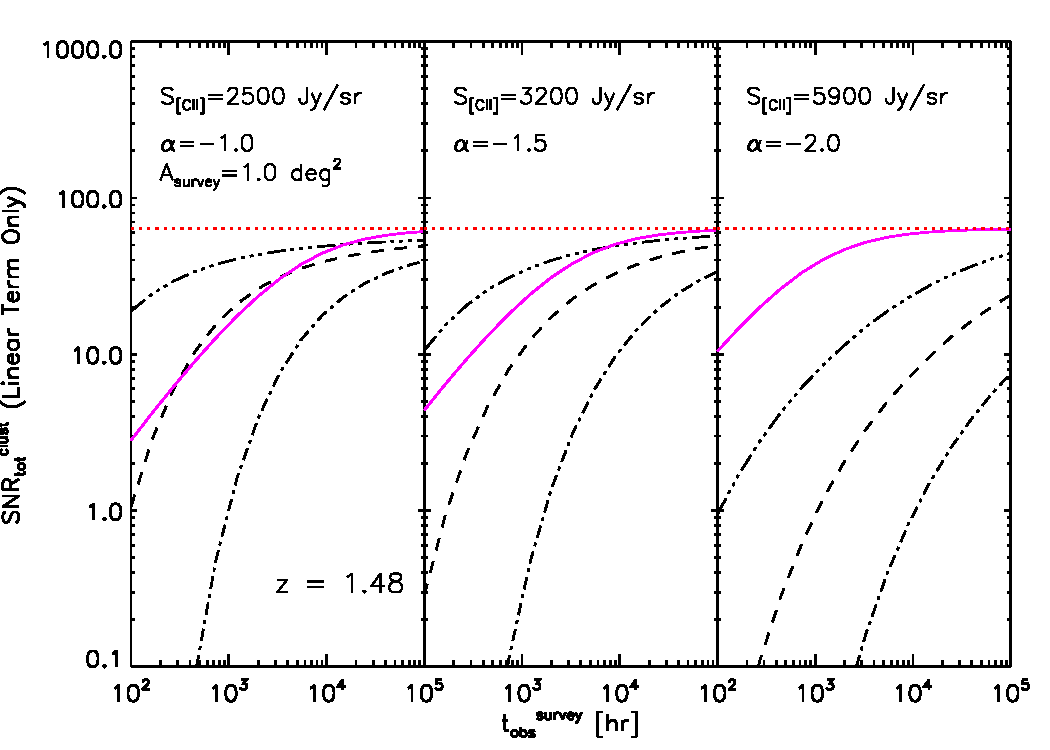
\includegraphics[width=0.5\textwidth]{SNRtot_starfire_cii_1sqdeg_z1p5_tsurvey_alpham_im_VpixR450_0p1Vpix_10Vpix_Lstar1d12_Lmin1d8_Lmax1d13}
\caption{Total Signal-to-Noise ratio ($\textrm{SNR}_{tot}$) on the linear portion of the clustering power spectrum of [CII] at $z=1.5$ as a function of the survey observing time (in hours). $\textrm{SNR}_{tot}$ as computed from intensity mapping---which depends only on the integral of the luminosity function, and not the shape---and from the Schechter function models are plotted. Magenta curves represent the intensity mapping experiment. Black Triple-dot-dashed, dashed, and dot-dashed lines correspond to galaxy survey experiments with pixel volumes 0.1, 1.0, 10.0 times the fiducial value. The horizontal dotted \emph{red line} is the maximum SNR, set by the number of modes in the survey volume. Note that the mean [CII] intensity is increasing for decreasing faint-end slopes, which is a consequence of fixing the total IR light for a given Schechter model to the B11 value, and then applying the $L_{[CII]}-L_{IR}$ relation to predict [CII] luminosity.}
 \label{fig:snr_vs_time_z1p5}
\end{figure}

\begin{figure*}[h]
 \centering
 \subfloat{
 \label{}
 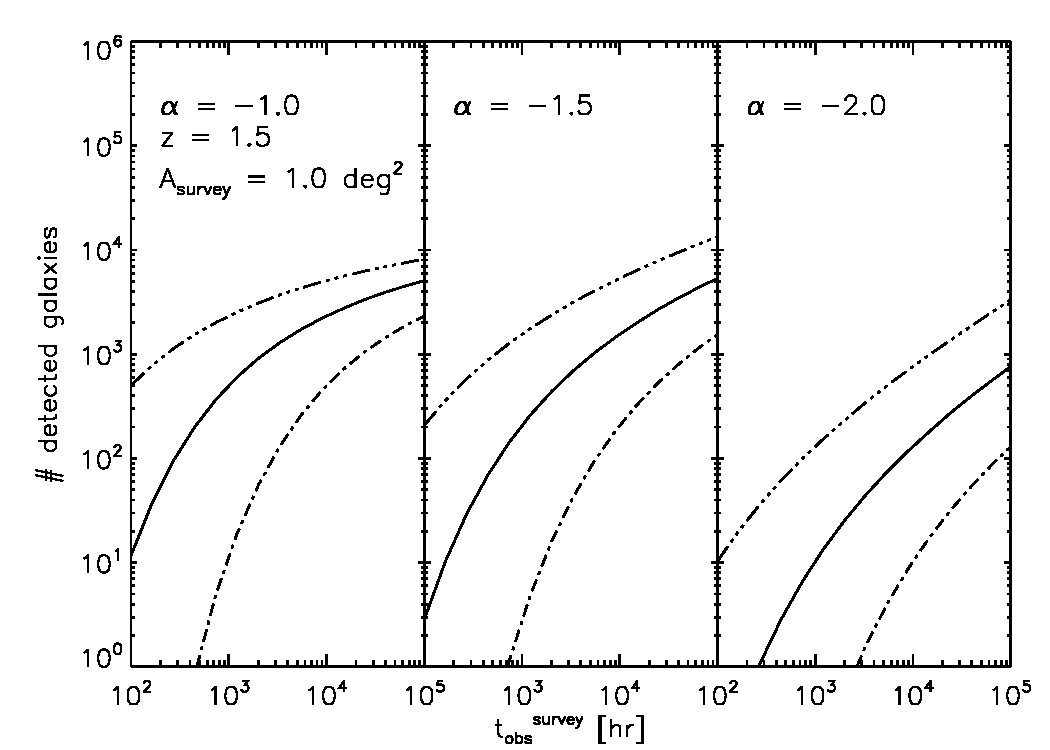
\includegraphics[width=0.5\textwidth]{Ngal_cii_STARFIRE_1sqdeg_z1p5_tsurvey_0p1vpix_vpix_10vpix_alpham1p0_alpham1p5_alpham2p0}}
 \subfloat{
 \label{}
 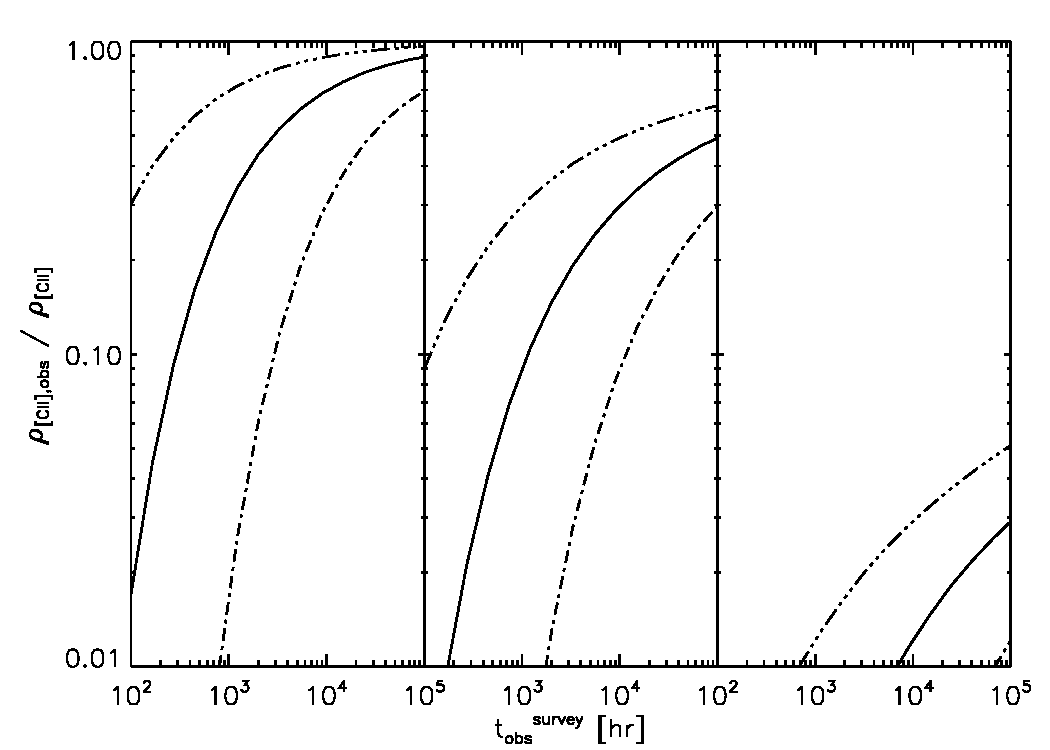
\includegraphics[width=0.5\textwidth]{frac_cii_STARFIRE_1sqdeg_z1p5_tsurvey_0p1vpix_vpix_10vpix_alpham1p0_alpham1p5_alpham2p0}}
 \centering
\caption{The predicted number of [CII]-detected galaxies and observed fraction of [CII] intensity as a function of observing time for the square degree field. Solid, dash-triple-dotted, and dash-dotted curves represent the fiducial $V_{pix}$, $0.1V_{pix}$, and $10 V_{pix}$, resp.}
\label{fig:ngal_frac}
\end{figure*}

\section{Discussion}

Should mention here implications for high redshift, CCAT, and future NASA FIR surveyor missions (SAFIR?)

\section{Summary}

We have presented predictions for the measurement of the [CII] power spectrum between $0.63 < z < 1.48$, and demonstrated the detectability of the power spectrum in both clustering and shot noise terms in this redshift range. Fluctuations of [CII] intensity have been modeled by combining empirically-constrained estimates of the [CII] luminosity from the B11 IR luminosity function and Spinoglio et al $L_i-L_{IR}$ relations with the theorized dark matter power spectrum. On large scales, the fact that the clustering amplitude of [CII] fluctuations is proportional to the mean [CII] intensity indicates the potential for measuring cosmic evolution of aggregate [CII] emission with the line intensity mapping approach. For the fiducial experiment considered in this paper, we have found that it would be possible to measure the [CII] luminosity density with fractional errors on the order of 10\%. We have further demonstrated that intensity mapping experiments always outperform galaxy redshift surveys when measuring the mean [CII] intensity and, for steep luminosity functions, clustering power spectrum, as well.



\appendix

Schechter function details

\bibliography{master_references}



\end{document}







